\documentclass[journal,12pt,onecolumn]{IEEEtran}
\usepackage{amsmath,amssymb,amsfonts,amsthm}
\usepackage{graphicx}
\usepackage{enumitem}
\usepackage[breaklinks=true]{hyperref}
\usepackage{caption}
\usepackage{array}
\newtheorem{problem}{Problem}
\renewcommand{\thefigure}{\theenumi}
\renewcommand{\thetable}{\theenumi}


\usepackage{amsmath} 
\newcommand{\myvec}[1]{\begin{bmatrix}#1\end{bmatrix}}

\begin{document}

\title{GATE XE 2019}
\author{AI25BTECH11003 - Bhavesh Gaikwad}
\maketitle

%------------------------GENERAL APTITUDE------------------

\section*{General Aptitude}
\vspace{1cm}

\begin{enumerate}[label=\arabic*)]


\item Once the team of analysts identify the problem, we \_\_\_\_\_\_\_\_\_ in a better position to comment on the issue. Which one of the following choices CANNOT fill the given blank?
\hfill\raisebox{-1.5ex}{(GATE 2019 XE)} \\

\vspace{0.2cm}
\begin{enumerate}[label=\alph*)]
\item will be
\item were to be
\item are going to be
\item might be
\end{enumerate}

\vspace{0.5cm}

\item A final examination is the \underline{\hspace{2cm}} of a series of evaluations that a student has to go through.
\vspace{0.2cm}
\hfill\raisebox{-2.5ex}{(GATE 2019 XE)} \\

\begin{enumerate}[label=\alph*)]
\item culmination
\item consultation
\item desperation
\item insinuation
\end{enumerate}

\vspace{0.5cm}

\item If \texttt{IMHO = JNIP}; \texttt{IDK = JEL}; and \texttt{SO = TP}, then \texttt{IDC} = \underline{\hspace{2cm}}.
\hfill\raisebox{-1.5ex}{(GATE 2019 XE)} \\

\vspace{0.2cm}
\begin{enumerate}[label=\alph*)]
\item JDE
\item JED
\item JDC
\item JCD
\end{enumerate}

\vspace{0.5cm}

\item The product of three integers $X$, $Y$ and $Z$ is $192$. $Z$ is equal to $4$ and $P$ is equal to the average of $X$ and $Y$. What is the minimum possible value of $P$?
\hfill\raisebox{-1.5ex}{(GATE 2019 XE)} \\

\vspace{0.2cm}
\begin{enumerate}[label=\alph*)]
\item 6
\item 7
\item 8
\item 9.5
\end{enumerate}

\vspace{0.5cm}

\item Are there enough seats here? There are \underline{\hspace{2cm}} people here than I expected.
\hfill\raisebox{-1.5ex}{(GATE 2019 XE)} \\

\vspace{0.2cm}
\begin{enumerate}[label=\alph*)]
\item many
\item most
\item least
\item more
\end{enumerate}

\vspace{0.5cm}

\item Fiscal deficit was $4\%$ of the GDP in 2015 and that increased to $5\%$ in 2016. If the GDP increased by $10\%$ from 2015 to 2016, the percentage increase in the actual fiscal deficit is \underline{\hspace{2cm}}.
\vspace{0.2cm}
\hfill\raisebox{-1.5ex}{(GATE 2019 XE)} \\

\begin{enumerate}[label=\alph*)]
\item 37.50
\item 35.70
\item 25.00
\item 10.00
\end{enumerate}

\vspace{0.5cm}

\item Two pipes $P$ and $Q$ can fill a tank in $6$ hours and $9$ hours respectively, while a third pipe $R$ can empty the tank in $12$ hours. Initially, $P$ and $R$ are open for $4$ hours. Then $P$ is closed and $Q$ is opened. After $6$ more hours $R$ is closed. The total time taken to fill the tank (in hours) is \underline{\hspace{2cm}}.
\vspace{0.2cm}
\hfill\raisebox{-1.5ex}{(GATE 2019 XE)} \\

\begin{enumerate}[label=\alph*)]
\item 13.50
\item 14.50
\item 15.50
\item 16.50
\end{enumerate}

\vspace{0.5cm}

\item While teaching a creative writing class in India, I was surprised at receiving stories from the students that were all set in distant places: in the American West with cowboys and in Manhattan penthouses with clinking ice cubes. This was, till an eminent Caribbean writer gave the writers in the once-colonised countries the confidence to see the shabby lives around them as worthy of being ``told''. The writer of this passage is surprised by the creative writing assignments of his students, because
\vspace{0.2cm}
\hfill\raisebox{-1.5ex}{(GATE 2019 XE)} \\

\begin{enumerate}[label=\alph*)]
\item Some of the students had written stories set in foreign places
\item None of the students had written stories set in India
\item None of the students had written about ice cubes and cowboys
\item Some of the students had written about ice cubes and cowboys
\end{enumerate}

\vspace{0.5cm}

\item Mola is a digital platform for taxis in a city. It offers three types of rides -- Pool, Mini and Prime. The Table below presents the number of rides for the past four months. The platform earns one US dollar per ride. What is the percentage share of revenue contributed by Prime to the total revenues of Mola, for the entire duration?

\vspace{0.5em}

\begin{center}
\begin{tabular}{ll}
    \textbf{Group I} & \textbf{Group II} \\
    P. Ferrite & 1. Hexagonal Close Packed (HCP) \\
    Q. Austenite & 2. Body Centered Cubic (BCC) \\
    R. Martensite & 3. Body Centered Tetragonal (BCT) \\
    & 4. Face Centered Cubic (FCC)
\end{tabular}
\end{center}

\hfill\raisebox{-1.5ex}{(GATE 2019 XE)} \\

\vspace{0.2cm}
\begin{enumerate}[label=\alph*)]
\item 16.24
\item 23.97
\item 25.86
\item 38.74
\end{enumerate}

\vspace{0.5cm}

\item X is an online media provider. By offering unlimited and exclusive online content at attractive prices for a loyalty membership, X is almost forcing its customers towards its loyalty membership. If its loyalty membership continues to grow at its current rate, within the next eight years more households will be watching X than cable television. Which one of the following statements can be inferred from the above paragraph?
\hfill\raisebox{-1.5ex}{(GATE 2019 XE)} \\

\vspace{0.2cm}
\begin{enumerate}[label=\alph*)]
\item Most households that subscribe to X’s loyalty membership discontinue watching cable television
\item Non-members prefer to watch cable television
\item Cable television operators don’t subscribe to X’s loyalty membership
\item The X is canceling accounts of non-members
\end{enumerate}

\end{enumerate}

\vspace{3\baselineskip}
\begin{center}
    \item[\textbf{END OF SECTION- GA}]
\end{center}





%---------------------SECTION-A---------------

\newpage
\section*{Engineering Mathematics}
\noindent
\vspace{1cm}

\begin{enumerate}[label=\arabic*)]
\item Let $X$ be the Poisson random variable with parameter $\lambda=1$. Then, the probability $P(2 \le X \le 4)$ equals
\hfill\raisebox{-1.5ex}{(GATE 2019 XE)} \\

\vspace{0.2cm}
\begin{enumerate}[label=\alph*)]
\item $\dfrac{19}{24e}$
\vspace{0.1cm}
\item $\dfrac{17}{24e}$
\vspace{0.1cm}
\item $\dfrac{13}{24e}$
\vspace{0.1cm}
\item $\dfrac{11}{24e}$
\end{enumerate}

\vspace{0.5cm}

\item For the series $\sum_{n=1}^{\infty}\dfrac{(x+1)^n}{n,2^n}$, $-\infty<x<\infty$, which of the following statements is NOT correct?
\vspace{0.1cm}
\hfill\raisebox{-1.5ex}{(GATE 2019 XE)} \\

\begin{enumerate}[label=\alph*)]
\item The series converges at $x=-3$
\item The series converges at $x=-1$
\item The series converges at $x=0$
\item The series converges at $x=1$
\end{enumerate}

\vspace{0.5cm}

\item Let $f(z)=\bar{z}, e^{-|z|^2}$, where $\bar{z}$ is the complex conjugate of $z$. Then, it is differentiable on
\hfill\raisebox{-2.5ex}{(GATE 2019 XE)} \\

\vspace{0.2cm}
\begin{enumerate}[label=\alph*)]
\item $|z|>1$
\item $|z|<1$
\item $|z|=1$
\item the entire complex plane $\mathbb{C}$
\end{enumerate}

\vspace{0.5cm}

\item If the transformation $u(x,t)=e^{-x},v(x,t)$ reduces the partial differential equation $\dfrac{\partial^2 u}{\partial x^2}-2\dfrac{\partial u}{\partial x}+u=9$ to the equation $\dfrac{\partial^2 v}{\partial x^2}=9,f(x)$, then $f(x)$ equals
\hfill\raisebox{-2.5ex}{(GATE 2019 XE)} \\

\vspace{0.2cm}
\begin{enumerate}[label=\alph*)]
\item $-e^{-x}$
\item $e^{-x}$
\item $-2e^{-x}$
\item $2e^{-x}$
\end{enumerate}

\newpage

\item The value of $\alpha$ for which the system of equations\\
$x-y-3z=3$\\
$2x+z=0$\\
$-2y-7z=\alpha$\\
 has a solution is \underline{\hspace{2cm}}.

\hfill\raisebox{-1.5ex}{(GATE 2019 XE)} \\
\vspace{1.0cm}

\item The value of the line integral $\displaystyle \oint_{\gamma}(-y^3dx + x^3dy)$, where $\gamma$ is the circle $x^2+y^2=1$ oriented counter clockwise, is \underline{\hspace{2cm}}.

\vspace{0.5cm}

\item Let $y_1(x)$ and $y_2(x)$ be two linearly independent solutions of the differential equation $x^2y''+xy'-4y=0$, $x>0$. If $y_1(x)=x^2$, then $\displaystyle \lim_{x\to\infty} y_2(x)$ is \underline{\hspace{2cm}}.
\hfill\raisebox{-1.5ex}{(GATE 2019 XE)} \\

\vspace{0.5cm}

\item If 
$Q = \myvec{3 & 2 & 4 \\ 2 & 0 & 2 \\ 4 & 2 & 3}$ and $P=(\mathbf{v}_1\ \mathbf{v}_2\ \mathbf{v}_3)$ is the matrix where $\mathbf{v}_1, \mathbf{v}_2$ and $\mathbf{v}_3$ are linearly independent eigenvectors of the matrix $Q$, then the sum of the absolute values of all the elements of the matrix $P^{-1}QP$ is
\hfill\raisebox{-1.5ex}{(GATE 2019 XE)} \\

\vspace{0.2cm}
\begin{enumerate}[label=\alph*)]
\item 6
\item 10
\item 14
\item 22
\end{enumerate}

\vspace{0.5cm}

\item If $P(x)=a x^3+b x^2+c x+d$ is the polynomial obtained by Lagrange interpolation satisfying $P(0)=-8$, $P(1)=-7$, $P(2)=-6$ and $P(4)=20$, then the value of $a-b+c$ is
\hfill\raisebox{-2.5ex}{(GATE 2019 XE)} \\

\vspace{0.2cm}
\begin{enumerate}[label=\alph*)]
\item 1
\item 3
\item 5
\item 7
\end{enumerate}

\vspace{0.5cm}

\item The number of critical points of the function $f(x,y)=x^3+3xy^2-15x-12y$ at which there is neither maximum nor minimum is \underline{\hspace{2cm}}.
\hfill\raisebox{-2.5ex}{(GATE 2019 XE)} \\

\vspace{0.5cm}

\item Let $I=\dfrac{10^5i}{2\pi}\oint_{\gamma}\dfrac{dz}{(z-4)(z^7-1)}$, where $i=\sqrt{-1}$ and $\gamma$ is the circle $|z|=2$ oriented counter clockwise. Then, the value of $I$ rounded off to one decimal place is \underline{\hspace{2cm}}.
\hfill\raisebox{-2.5ex}{(GATE 2019 XE)} \\

\end{enumerate}

\vspace{2\baselineskip}
\begin{center}
    \item[\textbf{END OF SECTION- A}]
\end{center}


\newpage

%-----------------SECTION-B-----------

\section*{Fluid Mechanics}
\noindent
\vspace{1cm}

\begin{enumerate}[label=\arabic*)]
\item For stable equilibrium of a floating body, which one of the following statements is correct?
\hfill\raisebox{-2.5ex}{(GATE 2019 XE)} \\

\vspace{0.2cm}
\begin{enumerate}[label=\alph*)]
\item Centre of gravity must be located below the centre of buoyancy.
\item Centre of buoyancy must be located below the centre of gravity.
\item Metacentre must be located below the centre of gravity.
\item Centre of gravity must be located below the metacentre.
\end{enumerate}

\vspace{0.5cm}

\item If $u$ and $v$ are the velocity components in the $x$- and $y$-directions respectively, the $z$-component of vorticity $\omega_z$ at a point in a flow field is
\hfill\raisebox{-1.5ex}{(GATE 2019 XE)} \\

\vspace{0.2cm}
\begin{enumerate}[label=\alph*)]
\item $\dfrac{\partial v}{\partial x}-\dfrac{\partial u}{\partial y}$
\item $\dfrac{\partial u}{\partial x}-\dfrac{\partial v}{\partial y}$
\item $\dfrac{\partial v}{\partial y}+\dfrac{\partial u}{\partial x}$
\item $\dfrac{\partial u}{\partial y}-\dfrac{\partial v}{\partial x}$
\end{enumerate}

\vspace{0.5cm}

\item In which one of the following devices the difference between static and total pressure is used to determine the flow velocity?
\hfill\raisebox{-1.5ex}{(GATE 2019 XE)} \\

\vspace{0.2cm}
\begin{enumerate}[label=\alph*)]
\item Piezometer
\item Pitot static tube
\item Orificemeter
\item Venturimeter
\end{enumerate}

\vspace{0.5cm}

\item A golf ball is dimpled to make the flow turbulent and consequently to reduce the drag. Turbulent flow reduces the drag on the golf ball because
\hfill\raisebox{-1.5ex}{(GATE 2019 XE)} \\

\vspace{0.2cm}
\begin{enumerate}[label=\alph*))]
\item skin friction coefficient is lower in a turbulent flow.
\item skin friction coefficient is higher in a turbulent flow.
\item turbulent flow has a lower tendency to separate.
\item turbulent flow has a higher tendency to separate.
\end{enumerate}

\vspace{0.5cm}

\item For a steady laminar incompressible boundary layer flow over a sharp-edged flat plate at zero incidence,
\hfill\raisebox{-1.5ex}{(GATE 2019 XE)} \\

\vspace{0.2cm}
\begin{enumerate}[label=\alph*)]
\item the edge of the boundary layer is a streamline.
\item the edge of the boundary layer is a pathline.
\item the skin friction coefficient decreases as the distance from the leading edge increases.
\item the skin friction coefficient remains constant all along the plate.
\end{enumerate}

\vspace{0.5cm}

\item The power input $P$ to a centrifugal pump is a function of the volume flow rate $Q$, impeller diameter $D$, rotational speed $\Omega$, fluid density $\rho$, dynamic viscosity $\mu$, and surface roughness $\varepsilon$. To carry out a dimensional analysis using Buckingham’s $\pi$ theorem, which one of the following sets can be taken as the set of repeating variables?
\hfill\raisebox{-1.5ex}{(GATE 2019 XE)} \\

\vspace{0.2cm}
\begin{enumerate}[label=\alph*)]
\item $Q,\ \Omega,\ D$
\item $Q,\ \varepsilon,\ D$
\item $\varepsilon,\ D,\ \rho$
\item $D,\ \rho,\ \Omega$
\end{enumerate}

\vspace{0.5cm}

\item Consider the two-dimensional laminar flow of water ($\mu=0.001\ \mathrm{N\cdot s/m^2}$) between two infinitely long parallel plates $0.1\ \mathrm{m}$ apart as shown in the figure below. The velocity profile at any location is given by $u(y)=100(0.1y-y^2)$ m/s where $y$ is in m. The magnitude of shear stress (in N/m$^2$, rounded off to 2 decimal places) acting on the bottom plate is \underline{\hspace{2cm}}.

\begin{figure}[htbp]
  \centering
  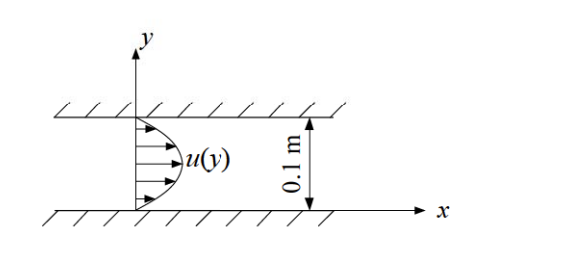
\includegraphics[width=.7\linewidth]{figs/B/fig1.png}
  \caption{Laminar flow of water}
  \label{B/fig1}
\end{figure}

\hfill\raisebox{-1.5ex}{(GATE 2019 XE)} \\

\vspace{0.5cm}

\item The maximum velocity in a fully developed laminar incompressible flow through a circular pipe of constant cross-sectional area is $6\ \mathrm{m/s}$. The average velocity (in m/s) of the flow is \underline{\hspace{2cm}}.
\vspace{0.2cm}
\hfill\raisebox{-1.5ex}{(GATE 2019 XE)} \\

\vspace{0.5cm}

\item The theoretical discharge for the flow through an orificemeter is $40\ \mathrm{m^3/s}$. If the measured discharge in an experiment is $32\ \mathrm{m^3/s}$, then the discharge coefficient (rounded off to one decimal place) is \underline{\hspace{2cm}}.
\hfill\raisebox{-1.5ex}{(GATE 2019 XE)} \\

\vspace{0.5cm}

\item Consider the flow between two infinitely long parallel plates of large width separated by a distance $2H$. The upper plate is moving with a constant velocity $U$ while the lower plate is stationary. The volumetric flow rate per unit width of the plate is
\hfill\raisebox{-1.5ex}{(GATE 2019 XE)} \\

\vspace{0.1cm}
\begin{enumerate}[label=\alph*)]
\item $0.25, U H$
\item $0.5, U H$
\item $U H$
\item $2, U H$
\end{enumerate}

\vspace{0.5cm}

\item The velocity field in Cartesian coordinates in a two-dimensional steady incompressible flow of a fluid with density $\rho$ is $\mathbf{V} = x,\hat{\imath} - y,\hat{\jmath}$. Assuming no body and line forces, the magnitude of pressure gradient $\nabla p$ at point $(1,1)$ is
\hfill\raisebox{-1.5ex}{(GATE 2019 XE)} \\

\vspace{0.2cm}
\begin{enumerate}[label=\alph*)]
\item $\sqrt{2},\rho$
\item $\rho$
\item $\rho/\sqrt{2}$
\item $\rho/2$
\end{enumerate}

\vspace{0.5cm}

\item A two-dimensional velocity field in Cartesian coordinates is defined by $\mathbf{V} = y,\hat{\imath} - x,\hat{\jmath}$. This flow is
\hfill\raisebox{-1.5ex}{(GATE 2019 XE)} \\

\vspace{0.2cm}
\begin{enumerate}[label=\alph*)]
\item compressible and rotational
\item compressible and irrotational
\item incompressible and rotational
\item incompressible and irrotational
\end{enumerate}

\vspace{0.5cm}

\item \textbf{Assertion [A]:} The streamlines in a free vortex flow are concentric circles. \\
\textbf{Reasoning [R]:} There exists only radial component for the velocity field in a free vortex flow.
\vspace{0.2cm}
\hfill\raisebox{-1.5ex}{(GATE 2019 XE)} \\

\begin{enumerate}[label=\alph*)]
\item Both [A] and [R] are true and [R] is the correct reason for [A]
\item Both [A] and [R] are true but [R] is not the correct reason for [A]
\item [A] is true but [R] is false
\item [A] is false but [R] is true
\end{enumerate}

\vspace{0.5cm}

\item The velocity components in Cartesian coordinates in a two-dimensional incompressible flow are $u=e^{x}\cos x$ and $v=e^{x}\sin x$. The magnitude of total acceleration at the point $(-1,1)$ is
\hfill\raisebox{-1.5ex}{(GATE 2019 XE)} \\

\vspace{0.2cm}
\begin{enumerate}[label=\alph*)]
\item 0
\item 1
\item $e$
\item $e^2$
\end{enumerate}

\vspace{0.3cm}

\item For steady laminar flow at zero incidence over a flat plate, the component of velocity parallel to the plate in the boundary layer is given by $u(y)=a+b y+c y^2$, where $y$ is the distance measured normal to the flat plate. If $\mu$ is the coefficient of dynamic viscosity, $U$ is the velocity parallel to the wall at the edge of the boundary layer and $\delta$ is the boundary layer thickness, the wall shear stress is given by
\hfill\raisebox{-0.5ex}{(GATE 2019 XE)} \\

\vspace{0.1cm}
\begin{enumerate}[label=\alph*)]
\item $\mu,U/\delta$
\item $2\mu,U/\delta$
\item $2\mu,(U/\delta)^2$
\item $3\mu,U/\delta$
\end{enumerate}

\newpage

\item A fluid with constant density of $1\ \mathrm{kg/m^3}$ flows past a semi-cylindrical structure with a freestream velocity of $2\ \mathrm{m/s}$ as shown in the figure below. The difference in static pressure between points $P$ and $Q$ is $10\ \mathrm{N/m^2}$. If the gravitational acceleration $g$ is $10\ \mathrm{m/s^2}$ and the flow is assumed to be potential, what is the radius $r$ (in m) of the semi-cylindrical structure?

\begin{figure}[htbp]
  \centering
  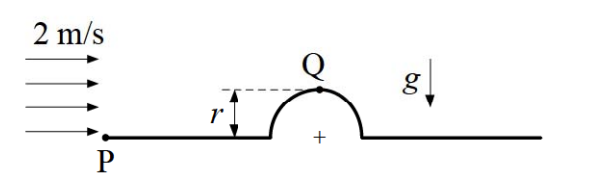
\includegraphics[width=.55\linewidth]{figs/B/fig2.png}
  \caption{Diagram}
  \label{B/fig2}
\end{figure}
\hfill\raisebox{-0.5ex}{(GATE 2019 XE)} \\

\vspace{0.2cm}
\begin{enumerate}[label=\alph*)]
\item 1
\item 0.8
\item 0.6
\item 0.4
\end{enumerate}



\vspace{0.5cm}

\item The mercury manometer shown in the figure below is connected to a water pipe at one end while the other end is open to the atmosphere. The density of water is $1000\ \mathrm{kg/m^3}$, the specific gravity of mercury is $13.6$ and the gravitational acceleration $g$ is $10\ \mathrm{m/s^2}$. The gauge pressure $p_w$ (in kN/m$^2$, rounded off to 2 decimal places) in the water pipe is \underline{\hspace{2cm}}.

\begin{figure}[htbp]
  \centering
  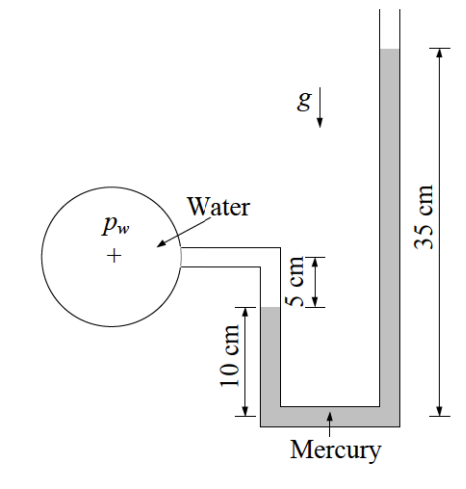
\includegraphics[width=.4\linewidth]{figs/B/fig3.png}
  \caption{Mercury Manometer}
  \label{B/fig3}
\end{figure}

\vspace{0.5cm}

\item Water ($\rho=1000\ \mathrm{kg/m^3}$, $\mu=0.001\ \mathrm{N\cdot s/m^2}$) flows through a smooth circular pipe of radius $0.05\ \mathrm{m}$. If the flow Reynolds number is $1000$, then the pressure drop (in N/m$^2$, rounded off to 2 decimals) over a length of $5\ \mathrm{m}$ will be \underline{\hspace{2cm}}.
\hfill\raisebox{-1.5ex}{(GATE 2019 XE)} \\

\vspace{0.5cm}

\item A uniform flow with a velocity of $2\ \mathrm{m/s}$ in the $x$-direction approaches a line source placed on the $x$-axis at a distance of $0.1\ \mathrm{m}$ from the origin. If the origin is the stagnation point in the resulting flow, the strength of the source (in m$^2$/s, rounded off to 2 decimals) is \underline{\hspace{2cm}}.
\hfill\raisebox{-2.5ex}{(GATE 2019 XE)} \\

\vspace{0.5cm}

\item In a steady incompressible flow of a fluid past a smooth stationary sphere, the drag force $F$ depends on the flow velocity $U$, diameter $D$, and the dynamic viscosity $\mu$ and density $\rho$ of the fluid. Experiments are conducted on the same sphere at the same flow velocity using two different fluids. The density of the second fluid is two times that of the first fluid. The dynamic viscosity of the second fluid is $n$ times that of the first fluid. If the non-dimensional force $\dfrac{F}{\rho U^2 D^2}$ remains the same in both the experiments, the value of $n$ is \underline{\hspace{2cm}}.
\hfill\raisebox{-1.5ex}{(GATE 2019 XE)} \\

\vspace{0.5cm}

\item An incompressible fluid flows past a flat plate as shown in the figure below with a uniform inlet velocity profile $u=U$ and a parabolic exit velocity profile $u=U(2\eta - \eta^2)$, where $u$ is the component of velocity parallel to the wall, $y$ is the normal distance from the plate and $\eta=y/\delta$. If the volume flow rate across the top surface of the control volume (CV) is $Q=p,U,\delta$ per unit width (perpendicular to the $x$-$y$ plane) of the plate, the value of $p$ (rounded off to 2 decimals) is \underline{\hspace{2cm}}.

\begin{figure}[htbp]
  \centering
  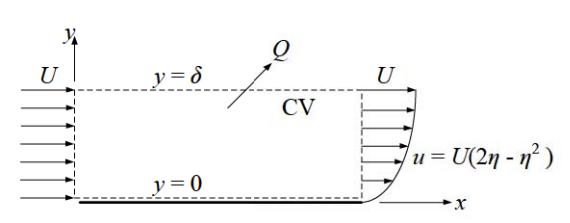
\includegraphics[width=.7\linewidth]{figs/B/fig4.png}
  \caption{Diagram}
  \label{B/fig4}
\end{figure}
\hfill\raisebox{-1.5ex}{(GATE 2019 XE)} \\

\newpage

\item A jet engine is to be tested on a thrust stand as shown in the figure below. The conditions prevailing in a typical test are as follows: Axial intake air velocity $=100\ \mathrm{m/s}$; axial exhaust gas velocity $=250\ \mathrm{m/s}$; intake cross-sectional area $=1\ \mathrm{m^2}$; intake static pressure $=-22\ \mathrm{kPa}$ (gauge); exhaust static pressure $=0\ \mathrm{kPa}$ (gauge); mass flow rate through the engine $=100\ \mathrm{kg/s}$. The anchoring force (in kN) in axial direction on the thrust stand is \underline{\hspace{2cm}}.

\begin{figure}[htbp]
  \centering
  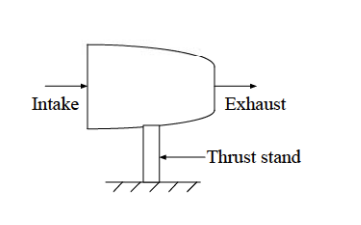
\includegraphics[width=.75\linewidth]{figs/B/fig5.png}
  \caption{Jet Engine}
  \label{B/fig5}
\end{figure}
\hfill\raisebox{-0.5ex}{(GATE 2019 XE)} \\

\end{enumerate}

\vspace{3\baselineskip}
\begin{center}
    \item[\textbf{END OF SECTION- B}]
\end{center}



%---------------------SECTION-C-------------------------

\newpage
\section*{Materials Science}
\noindent
\vspace{1cm}

\begin{enumerate}[label=\arabic*)]

\item On decreasing the objective aperture size in an optical microscope
\hfill\raisebox{-2.5ex}{(GATE 2019 XE)} \\

\vspace{0.2cm}
\begin{enumerate}[label=\alph*)]
\item the spherical aberration increases
\item the depth of field increases
\item the diffraction-limited resolution increases
\item the astigmatism increases
\end{enumerate}

\vspace{0.5cm}

\item Pilling-Bedworth ratios for oxides of some metals are given in the table.\\

\begin{tabular}{|c|c|c|}
     \hline
     \textbf{Mineral} & \textbf{Modal abundance \brak{\%}} & \textbf{Partition coefficient}\\
     \hline
     Clinopyroxene & $45$ & $0.506$ \\
      \hline
      Orthopyroxene & $40$ & $0.42$ \\
      \hline
      Olivine & $10$ & $0.045$ \\
      \hline
      Plagioclase & $05$ & $0.019$ \\
      \hline
\end{tabular}

Based on the criterion of Pilling-Bedworth ratio alone, which one of the following metals will be most protected from high temperature oxidation?
\hfill\raisebox{-2.5ex}{(GATE 2019 XE)} \\

\vspace{0.2cm}
\begin{enumerate}[label=\alph*)]
\item Li
\item Ce
\item Ta
\item W
\end{enumerate}

\vspace{0.5cm}

\item In NaCl, the substitution of a Na$^+$ ion by a Ca$^{2+}$ ion would most probably lead to
\hfill\raisebox{-2.5ex}{(GATE 2019 XE)} \\

\vspace{0.2cm}
\begin{enumerate}[label=\alph*)]
\item the formation of a Na$^+$ vacancy
\item the creation of a Cl$^-$ interstitial
\item the formation of a Cl$^-$ vacancy
\item the formation of a Na$^+$ and Cl$^-$ vacancy pair
\end{enumerate}

\vspace{0.5cm}

\item Which one of the following is time-independent?
\hfill\raisebox{-2.5ex}{(GATE 2019 XE)} \\

\vspace{0.2cm}
\begin{enumerate}[label=\alph*)]
\item Elastic deformation
\item Anelastic deformation
\item Viscoelastic deformation
\item Creep deformation
\end{enumerate}

\vspace{0.3cm}

\item Copper is diffused into aluminium at $400^\circ$C for 100 hours to obtain a certain concentration at a given depth. In another experiment conducted at $500^\circ$C, to achieve the same concentration of copper at the same depth, the time required in hours is (Given: Diffusion coefficients of copper in aluminium at $400^\circ$C and $500^\circ$C are $5\times10^{-14}\ \mathrm{m^2 s^{-1}}$ and $6\times10^{-13}\ \mathrm{m^2 s^{-1}}$, respectively)
\hfill\raisebox{-2.5ex}{(GATE 2019 XE)} \\

\vspace{0.5cm}

\item If carbon (C) in iron (Fe) is 6 percent by weight, then its atomic percent is approximately (Given: atomic weight C=12, Fe=56)
\hfill\raisebox{-2.5ex}{(GATE 2019 XE)} \\

\vspace{0.2cm}
\begin{enumerate}[label=\alph*)]
\item 13
\item 23
\item 30
\item 50
\end{enumerate}

\vspace{0.5cm}

\item GaAs has advantage over silicon when used in integrated circuits at low power because it has
\vspace{0.2cm}
\hfill\raisebox{-2.5ex}{(GATE 2019 XE)} \\

\begin{enumerate}[label=\alph*)]
\item larger band gap
\item more than one element
\item higher electron mobility
\item higher hole mobility
\end{enumerate}

\vspace{0.5cm}

\item Glass transition temperature of a polymer can be determined by
\hfill\raisebox{-2.5ex}{(GATE 2019 XE)} \\

\vspace{0.2cm}
\begin{enumerate}[label=\alph*)]
\item Thermo-gravimetric analysis
\item Raman spectroscopy
\item NMR spectroscopy
\item Differential scanning calorimetry
\end{enumerate}

\vspace{0.5cm}

\item The maximum wavelength of radiation to which Germanium (Ge) is opaque will be (Given: energy gap of Ge=0.67 eV, Planck's constant $h=6.63\times10^{-34}$ J$\cdot$s, velocity of light $c=3\times10^{8}$ m$\cdot$s$^{-1}$ and 1 eV$=1.6\times10^{-19}$ J)
\hfill\raisebox{-2.5ex}{(GATE 2019 XE)} \\

\vspace{0.2cm}
\begin{enumerate}[label=\alph*)]
\item 0.8 $\mu$m
\item 1.8 $\mu$m
\item 2.8 $\mu$m
\item 4.8 $\mu$m
\end{enumerate}

\vspace{0.5cm}

\item An alternating copolymer has number-averaged molecular weight of $10^{5}$ g$\cdot$mol$^{-1}$ and degree of polymerization of 2210. If one of the repeat units is ethylene, the other one is (Given: atomic weight of H=1, C=12, F=19 and Cl=35.5)
\hfill\raisebox{-2.5ex}{(GATE 2019 XE)} \\

\vspace{0.2cm}
\begin{enumerate}[label=\alph*)]
\item --CH$_2$--CH(CH$_3$)--
\item --CH$_2$--CHCl--
\item --CF$_2$--CF$_2$--
\item --CH$_2$--CH(C$_6$H$_5$)--
\end{enumerate}

\newpage

\item Match the sintering processes in column I with the most suitable products in column II.\\

\begin{table}[htbp]
  \centering
  \caption{Table-3}
  \label{table3}
  \begin{tabular}{cc}
  \textbf{Processing Technique} & \textbf{Producct} \\ \\
    P. Calendering & 1. Pipes \\
    Q. Extrusion & 2. Disposable cups \\
    R. Injection moulding & 3. Sheets \\
    S. Thermoforming & 4. Nylon gears \\
  \end{tabular}
\end{table}

\vspace{0.2cm}
\hfill\raisebox{-2.5ex}{(GATE 2019 XE)} \\

\begin{enumerate}[label=\alph*)]
\item P-4; Q-1; R-2; S-3
\item P-3; Q-2; R-1; S-4
\item P-3; Q-2; R-4; S-1
\item P-2; Q-3; R-1; S-4
\end{enumerate}

\vspace{0.5cm}

\item Which one of the following conditions will NOT favour the separation of impurities in zone refining process?
\hfill\raisebox{-2.5ex}{(GATE 2019 XE)} \\

\vspace{0.2cm}
\begin{enumerate}[label=\alph*)]
\item Increase in the gap between solidus and liquidus lines
\item Increase in the solubility of impurities in solid as compared to that in liquid phase
\item Agitation of melt
\item Low cooling rate of melt
\end{enumerate}

\vspace{0.5cm}

\item A monochromatic X-ray beam of wavelength 0.154 nm is incident on a cubic crystal having lattice parameter $a=0.245$ nm. The diffraction angle (2$\theta$) for the first order reflection from a set of planes represented by the schematic plane below is \underline{\hspace{2cm}} degrees (round off to 1 decimal place).

\begin{figure}[htbp]
  \centering
  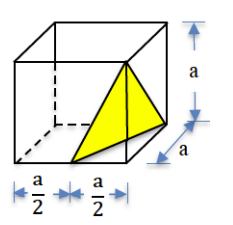
\includegraphics[width=.5\linewidth]{figs/C/fig1.png} 
  \caption{}
  \label{C/fig1}
\end{figure}

\hfill\raisebox{-2.5ex}{(GATE 2019 XE)} \\

\vspace{0.5cm}

\item Nickel corrodes at 298 K in a solution of 0.06 M nickel chloride having pH 4. Assuming complete dissociation of nickel chloride, the partial pressure of hydrogen required to stop the corrosion of nickel is \underline{\hspace{2cm}} atm (round off to the nearest integer)
\hfill\raisebox{-2.5ex}{(GATE 2019 XE)} \\

\vspace{0.5cm}

\item The potential energy, $U(r)$, of a pair of atoms spaced at a distance $r$ in a solid is given by $U(r)=-A/r^{3} + B/r^{7}$. The equilibrium distance between the atom pair is \underline{\hspace{2cm}} nm (round off to 2 decimal places)
\hfill\raisebox{-2.5ex}{(GATE 2019 XE)} \\

\vspace{0.5cm}

\item Tensile true stress–true strain curve for plastic region of an alloy is given by $\sigma(\text{MPa})=600,\varepsilon^{n}$. When true strain is 0.05, the true stress is 350 MPa. For the same alloy, when engineering strain is 0.12 then the engineering stress is \underline{\hspace{2cm}} MPa (round off to the nearest integer).
\hfill\raisebox{-2.5ex}{(GATE 2019 XE)} \\

\vspace{0.5cm}

\item Box-S has 2 white and 4 black balls and box-T has 5 white and 3 black balls. A ball is drawn at random, from the box-S and put in box-T. Subsequently, the probability of drawing a white ball from box-T is \underline{\hspace{2cm}} (round off to 2 decimal places).
\hfill\raisebox{-2.5ex}{(GATE 2019 XE)} \\

\vspace{0.5cm}

\item The zero point energy of an electron in a box of 0.2 nm width is \underline{\hspace{2cm}} eV (round off to 1 decimal place).
\hfill\raisebox{-1.5ex}{(GATE 2019 XE)} \\

\vspace{0.5cm}

\item The de Broglie wavelength of an electron accelerated across a 300 kV potential in an electron microscope is \underline{\hspace{2cm}}$\times10^{-12}$ m (round off to 2 decimal places). Ignore relativistic effects. (Given: Planck's constant=$6.63\times10^{-34}$ J$\cdot$s, electron rest mass=$9.11\times10^{-31}$ kg, electron charge=$1.6\times10^{-19}$)
\hfill\raisebox{-1.5ex}{(GATE 2019 XE)} \\

\vspace{0.5cm}

\item A stress of 17 MPa is applied to a polymer serving as a fastener in a complex assembly. At constant strain the stress drops to 16.6 MPa after 100 hours. The stress on the polymer must remain above 14.5 MPa in order for the assembly to function properly. The expected life of the assembly is \underline{\hspace{2cm}} hours (round off to the nearest integer).
\hfill\raisebox{-2.5ex}{(GATE 2019 XE)} \\


\item A piezoelectric material has a Young's modulus of 72 GPa. The stress required to change the polarization from 640 to 645 C$\cdot$mm$^{-3}$ is \underline{\hspace{2cm}} MPa (round off to the nearest integer).
\hfill\raisebox{-2.5ex}{(GATE 2019 XE)} \\

\vspace{0.5cm}

\item An iron bar magnet having coercivity of 7000 A$\cdot$m$^{-1}$ is to be demagnetized. The bar is introduced fully inside a 0.25 m long solenoid having 150 turns of wire. The electric current required to generate the necessary magnetic field is \underline{\hspace{2cm}} A (round off to 1 decimal place).
\hfill\raisebox{-2.5ex}{(GATE 2019 XE)} \\

\vspace{0.2cm}

\end{enumerate}

\begin{center}
    \item[\textbf{END OF SECTION- C}]
\end{center}

%------------------------------SECTION-D------------------

\newpage
\section*{Polymer Science}
\noindent
\vspace{1cm}
\begin{enumerate}[label=\arabic*)]

\item The functionality of allyl alcohol (CH$_2$=CH--CH$_2$OH) for condensation reaction with terephthalic acid is
\hfill\raisebox{-2.5ex}{(GATE 2019 XE)} \\

\vspace{0.2cm}
\begin{enumerate}[label=\alph*)]
\item 0
\item 1
\item 2
\item 3
\end{enumerate}

\vspace{0.5cm}

\item Which of the following polymers can be synthesized by ring opening polymerization?
\hfill\raisebox{-2.5ex}{(GATE 2019 XE)} \\

\vspace{0.2cm}
\begin{enumerate}[label=\alph*)]
\item Poly(vinyl alcohol)
\item Nylon 66
\item Poly(ethylene terephthalate)
\item Poly($\varepsilon$-caprolactone)
\end{enumerate}

\vspace{0.5cm}

\item The weather resistant polymer among the following is
\hfill\raisebox{-2.5ex}{(GATE 2019 XE)} \\

\vspace{0.2cm}
\begin{enumerate}[label=\alph*)]
\item natural rubber
\item styrene butadiene rubber
\item nitrile rubber
\item silicone rubber
\end{enumerate}

\vspace{0.5cm}

\item If a combination of sodium and naphthalene is used to initiate polymerization of styrene, then the most likely mechanism of polymerization is
\hfill\raisebox{-2.5ex}{(GATE 2019 XE)} \\

\vspace{0.2cm}
\begin{enumerate}[label=\alph*)]
\item free radical
\item cationic
\item anionic
\item olefin metathesis
\end{enumerate}

\vspace{0.5cm}

\item Hypalon is the trade name for
\hfill\raisebox{-2.5ex}{(GATE 2019 XE)} \\

\vspace{0.2cm}
\begin{enumerate}[label=\alph*)]
\item chlorosulfonated polyethylene
\item chlorinated polyethylene
\item ultra high molecular weight polyethylene
\item cross-linked polyethylene
\end{enumerate}

\vspace{0.5cm}

\item The copolymer(s) among high density polyethylene (HDPE), low density polyethylene (LDPE) and linear low density polyethylene (LLDPE) is/are
\hfill\raisebox{-2.5ex}{(GATE 2019 XE)} \\

\vspace{0.2cm}
\begin{enumerate}[label=\alph*)]
\item LDPE only
\item LLDPE only
\item LDPE and LLDPE
\item HDPE and LDPE
\end{enumerate}

\vspace{0.5cm}

\item The polymer which lacks the ability to exhibit tacticity among the following is
\hfill\raisebox{-2.5ex}{(GATE 2019 XE)} \\

\vspace{0.2cm}
\begin{enumerate}[label=\alph*)]
\item polypropylene
\item polystyrene
\item polyisobutylene
\item poly(methyl methacrylate)
\end{enumerate}

\vspace{0.5cm}

\item The correct order of glass transition temperature ($T_g$) for the polymers listed below is (PC=polycarbonate; PET=poly(ethylene terephthalate); PE=polyethylene; PP=polypropylene)
\hfill\raisebox{-2.5ex}{(GATE 2019 XE)} \\

\vspace{0.2cm}
\begin{enumerate}[label=\alph*)]
\item PC $>$ PET $>$ PP $>$ PE
\item PC $>$ PET $>$ PE $>$ PP
\item PET $>$ PC $>$ PE $>$ PP
\item PET $>$ PC $>$ PP $>$ PE
\end{enumerate}

\vspace{0.5cm}

\item Polystyrene coffee cup can be most economically manufactured by
\hfill\raisebox{-2.5ex}{(GATE 2019 XE)} \\

\vspace{0.2cm}
\begin{enumerate}[label=\alph*)]
\item thermoforming
\item injection molding
\item compression molding
\item blow molding
\end{enumerate}

\vspace{0.5cm}

\item Match the following rubber additives to their function:\\

\begin{center}
\begin{tabular}{|c|c|c|}
    \hline
    Task & Task time (Seconds) & Immediate predecessor(s) \\
    \hline
    P & 20 & - \\ \hline
    Q & 25 & P \\  \hline
    R & 10 & Q \\ \hline
    S & 15 & Q \\ \hline 
    T & 25 & R, S \\    \hline
\end{tabular}
\end{center}

\hfill\raisebox{-2.5ex}{(GATE 2019 XE)} \\

\vspace{0.2cm}
\begin{enumerate}[label=\alph*)]
\item P-4, Q-1, R-3, S-2
\item P-3, Q-1, R-4, S-2
\item P-3, Q-2, R-4, S-1
\item P-4, Q-2, R-3, S-1
\end{enumerate}

\newpage

\item Match the following polymers with their characteristic infrared (IR) stretching frequency:\\

\begin{table}[h!]
\centering
\begin{tabular}{|c|c|c|c|}
\hline
\textbf{Pressure} & \textbf{Temperature} & \multicolumn{2}{c|}{\textbf{Specific enthalpy}} \\ \cline{3-4} 
\textbf{(kPa)} & \textbf{($^\circ$C)} & $h_f$ (kJ/kg) & $h_g$ (kJ/kg) \\ \hline
150.9 & $-20$ & 17.82 & 178.74 \\ \hline
500 & 15.6 & 50.64 & 195.01 \\ \hline
\end{tabular}
\end{table}

\hfill\raisebox{-2.5ex}{(GATE 2019 XE)} \\
\vspace{0.2cm}
\begin{enumerate}[label=\alph*)]
\item P-2, Q-3, R-1, S-4
\item P-2, Q-1, R-4, S-3
\item P-4, Q-2, R-3, S-1
\item P-4, Q-1, R-2, S-3
\end{enumerate}

\vspace{0.5cm}

\item Match the following products to the most suitable polymer for their manufacture:\\

\begin{table}[htbp]
  \centering
  \caption{Table-6}
  \label{tab:tables/table6.tex}
  \begin{tabular}{cc}
  \textbf{Reagent} & \textbf{Function} \\ \\
    P.Ammonia  & 1. Prevent storage hardening \\
    Q. Hydroxylamine & 2. Delay plugging mechanism \\
    R. Formic acid & 3. Stabilizer \\
    S. Ethephone & 4. Coagulating agent \\
  \end{tabular}
\end{table}

\hfill\raisebox{-2.5ex}{(GATE 2019 XE)} \\

\vspace{0.2cm}
\begin{enumerate}[label=\alph*)]
\item P-3, Q-2, R-1, S-4
\item P-3, Q-4, R-2, S-1
\item P-4, Q-3, R-1, S-2
\item P-2, Q-3, R-1, S-4
\end{enumerate}

\vspace{0.5cm}

\item The order of limiting oxygen index for the following polymers is (PP=polypropylene; PTFE=polytetrafluoroethylene; PVC=poly(vinyl chloride))
\hfill\raisebox{-2.5ex}{(GATE 2019 XE)} \\

\vspace{0.2cm}
\begin{enumerate}[label=\alph*)]
\item PP $<$ PTFE $<$ Nylon 6 $<$ PVC
\item PP $<$ PVC $<$ Nylon 6 $<$ PTFE
\item PP $<$ Nylon 6 $<$ PVC $<$ PTFE
\item PP $<$ Nylon 6 $<$ PTFE $<$ PVC
\end{enumerate}

\newpage

\item Match the following plastic additives to their function:\\

\begin{table}[htbp]
  \centering
  \caption{Table-7}
  \label{tab:tables/table7.tex}
  \begin{tabular}{cc}
\textbf{Additives} & \textbf{Fuction}\\

P. Molybdenum disulphide & 1. Heat stabilizer \\
Q. Glycerol monostearate & 2. UV-absorber \\
R. Tribasic lead sulphate & 3. Antistatic agent \\
S. 2-hydroxybenzophenone & 4. Solid layer lubricant \\
  
  
  
  \end{tabular}
\end{table}

\hfill\raisebox{-2.5ex}{(GATE 2019 XE)} \\

\vspace{0.2cm}
\begin{enumerate}[label=\alph*)]
\item P-3, Q-1, R-2, S-4
\item P-3, Q-4, R-1, S-2
\item P-4, Q-3, R-2, S-1
\item P-4, Q-3, R-1, S-2
\end{enumerate}

\vspace{0.5cm}

\item Match the material classification in Column A with the appropriate one in Column B:\\
(PS=polystyrene, PPO=polyphenylene oxide, PDMS=poly(dimethyl siloxane), PP=polypropylene, PE=polyethylene, PP-g-MA=maleic anhydride grafted PP)\\

\begin{table}[htbp]
  \centering
  \caption{Table-8}
  \label{table8}
  \begin{tabular}{cc}
  \textbf{Group-I} & \textbf{Group-II} \\ \\
    P. Corn & 1. Lycopene \\
    Q. Red pepper & 2. $\beta$-Carotene \\
    R. Pumpkin & 3. Capsanthin \\
    S. Tomato & 4. Lutein \\
  \end{tabular}
\end{table}

\hfill\raisebox{-2.5ex}{(GATE 2019 XE)} \\

\vspace{0.2cm}
\begin{enumerate}[label=\alph*)]
\item P-3, Q-4, R-2, S-1
\item P-4, Q-3, R-2, S-1
\item P-3, Q-4, R-1, S-2
\item P-4, Q-3, R-1, S-2
\end{enumerate}

\vspace{0.5cm}

\item A linear amorphous polymer has a Tg of $+10^\circ$C. At $28^\circ$C, it has a melt viscosity of $4\times10^{8}$ poise. The viscosity of the polymer at its Tg is \underline{\hspace{2cm}}$\times10^{13}$ poise (round off to one decimal place).
\vspace{0.05cm}
\hfill\raisebox{-2.5ex}{(GATE 2019 XE)} \\

\vspace{0.5cm}

\item A polypropylene (PP) bar with a 10 mm$\times$10 mm square section is 225 mm long. The modulus of PP bar is 861 MN$\cdot$m$^{-2}$. It is pinned at both ends and an axial compressive load of 140 N is applied. The strain due to the applied load experienced by the PP bar is \underline{\hspace{2cm}}\% (round off to two decimal places).
\hfill\raisebox{-2.5ex}{(GATE 2019 XE)} \\

\newpage

\item In a unidirectional carbon fibre/vinyl ester composite, the ratio of the moduli of the carbon fibre to that of vinyl ester is 35 and the fibres take up 50\% of the cross-section. The percentage of applied force taken up by the fibres is \underline{\hspace{1cm}}\% (round off to one decimal place).

\hfill\raisebox{-0.5ex}{(GATE 2019 XE)} \\

\vspace{0.5cm}

\item A 3 mm thick layer of softened poly(methyl methacrylate) at $190^\circ$C is sandwiched between two flat parallel plates. A shear stress of 100 kPa is applied to the softened polymer. Assuming the softened polymer as a Newtonian fluid with an apparent viscosity of $3.9\times10^{4}$ Pa$\cdot$s, the relative sliding velocity between the two plates is \underline{\hspace{2cm}} mm$\cdot$s$^{-1}$ (round off to one decimal place).
\hfill\raisebox{-2.5ex}{(GATE 2019 XE)} \\

\vspace{0.5cm}

\item For AIBN initiated polymerization of styrene, if both the monomer and initiator concentration are doubled, then the rate of polymerization increases by a factor of \underline{\hspace{2cm}} (round off to two decimal places).
\hfill\raisebox{-2.5ex}{(GATE 2019 XE)} \\

\vspace{0.5cm}

\item If 49 moles of hexamethylene diamine is reacted with 50 moles of adipic acid to prepare Nylon 66, then the number average molecular weight, $M_{n}$, of the resulting polymer at 99.5\% conversion (ignoring contribution from end groups) is \underline{\hspace{2cm}} g$\cdot$mol$^{-1}$ (round off to 2 decimal places).
\vspace{0.05cm}
\hfill\raisebox{-2.5ex}{(GATE 2019 XE)} \\

\vspace{0.5cm}

\item A single screw extruder is to be used to manufacture a nylon rod of 0.5 cm diameter at a production rate of 2.5 cm$\cdot$s$^{-1}$. The density of solid nylon and nylon melt are 1.140 g$\cdot$cm$^{-3}$ and 0.790 g$\cdot$cm$^{-3}$, respectively. The melt flow rate through the die is \underline{\hspace{2cm}} cm$^{3}\cdot$s$^{-1}$ (round off to two decimal places).
\hfill\raisebox{-2.5ex}{(GATE 2019 XE)} \\

\vspace{0.5cm}

\end{enumerate}

\vspace{3\baselineskip}
\begin{center}
    \item[\textbf{END OF SECTION- D}]
\end{center}

%--------------------------SECTIOn-E-------------------

\newpage
\section*{Food Technology}
\noindent
\vspace{1cm}
\begin{enumerate}[label=\arabic*)]

\item Colloidal stability of milk casein is because of the highly hydrated carbohydrate residues in
\hfill\raisebox{-2.5ex}{(GATE 2019 XE)} \\

\vspace{0.2cm}
\begin{enumerate}[label=\alph*)]
\item $\alpha_{s1}$ casein
\item $\alpha_{s2}$ casein
\item $\beta$ casein
\item $\kappa$ casein
\end{enumerate}

\vspace{0.5cm}

\item Rice bran is stabilized prior to oil extraction to protect it from the activity of \underline{\hspace{2cm}}.
\hfill\raisebox{-2.5ex}{(GATE 2019 XE)} \\

\vspace{0.2cm}
\begin{enumerate}[label=\alph*)]
\item Polyphenol oxidase
\item Peroxidase
\item Lipase
\item Lipoxygenase
\end{enumerate}

\vspace{0.5cm}

\item Sticking of powder to wall of the chamber during spray drying of fruit juice is due to \underline{\hspace{2cm}}.
\vspace{0.05cm}
\hfill\raisebox{-2.5ex}{(GATE 2019 XE)} \\

\vspace{0.2cm}
\begin{enumerate}[label=\alph*)]
\item Low glass transition temperature of the compounds in juice
\item High glass transition temperature of the compounds in juice
\item Improper processing parameters of spray dryer
\item Presence of gums in feed material
\end{enumerate}

\vspace{0.5cm}

\item Thearubigins and theaflavins in black tea are formed by the oxidation and dimerization of
\hfill\raisebox{-2.5ex}{(GATE 2019 XE)} \\

\vspace{0.2cm}
\begin{enumerate}[label=\alph*)]
\item Quercetin
\item Catechins
\item Gallic acid
\item Kaempferol
\end{enumerate}

\vspace{0.5cm}

\item Ratio of Schmidt number to Lewis number is \underline{\hspace{2cm}}.
\hfill\raisebox{-2.5ex}{(GATE 2019 XE)} \\

\vspace{0.2cm}
\begin{enumerate}[label=\alph*)]
\item Prandtl number
\item Reynolds number
\item Nusselt number
\item Sherwood number
\end{enumerate}

\newpage

\item `Red dog' is one of the byproducts during milling of \underline{\hspace{2cm}}.
\hfill\raisebox{-2.5ex}{(GATE 2019 XE)} \\

\vspace{0.2cm}
\begin{enumerate}[label=\alph*)]
\item Corn
\item Rice
\item Ragi
\item Wheat
\end{enumerate}

\vspace{0.5cm}

\item An ice cream mix of 870 g$\cdot$L$^{-1}$ has been used to prepare ice cream which yielded a finished product of 490 g$\cdot$L$^{-1}$. The per cent over run is \underline{\hspace{2cm}} (round off to 1 decimal place).
\hfill\raisebox{-2.5ex}{(GATE 2019 XE)} \\

\vspace{0.5cm}

\item Impeller in a fruit juice mixing tank is rotating at 200 rpm with a Reynolds number $>10^{4}$. Density of juice is 1,045 kg$\cdot$m$^{-3}$. If diameter of the impeller is doubled and other conditions remained constant, the power requirement of mixing will increase by a factor of \underline{\hspace{2cm}}.
\hfill\raisebox{-2.5ex}{(GATE 2019 XE)} \\

\vspace{0.5cm}

\item Paddy consisting of 20\% husk has been milled to remove 6\% bran during polishing. Assuming no other losses, yield (per cent) of polished rice from the paddy is \underline{\hspace{2cm}} (round off to 1 decimal place).
\hfill\raisebox{-2.5ex}{(GATE 2019 XE)} \\

\vspace{0.5cm}

\item Match the following laws in Column I with corresponding phenomenon in Column II.\\

\begin{table}[htbp]
  \centering
  \caption{Table-9}
  \label{tab:tables/table9.tex}
  \begin{tabular}{cc}
  \textbf{Group-I} & \textbf{Group-II} \\ \\
    P. Degumming & 1. Crystallization of triacylglycerol by cooling to remove fat crystals \\
    Q. Deacidifying & 2. Passing heated oil over charcoal \\
    R. Bleaching & 3. Using alkaline solution to remove fatty acids \\
    S. Winterizing & 4. Wetting with water to remove lecithin \\
  \end{tabular}
\end{table}

\hfill\raisebox{-2.5ex}{(GATE 2019 XE)} \\

\vspace{0.2cm}
\begin{enumerate}[label=\alph*)]
\item P-2, Q-3, R-4, S-1
\item P-3, Q-2, R-4, S-1
\item P-3, Q-1, R-4, S-2
\item P-4, Q-3, R-2, S-1
\end{enumerate}

\newpage

\item Match the mold in Column I with its asexual/sexual spore shown in Column II.\\

\begin{table}[htbp]
  \centering
  \caption{Table-10}
  \label{table10}
  \begin{tabular}{cc}
\textbf{Column-I} & \textbf{Column-II}\\

P. Aspergillus & 1. Arthrospore \\
Q. Geotrichum & 2. Oospores \\
R. Rhizopus & 3. Conidia \\
S. Oomycetes & 4. Sporangiospores \\
  
  
  
  \end{tabular}
\end{table}
\hfill\raisebox{-2.5ex}{(GATE 2019 XE)} \\

\vspace{0.2cm}
\begin{enumerate}[label=\alph*)]
\item P-3, Q-1, R-4, S-2
\item P-1, Q-4, R-3, S-2
\item P-4, Q-3, R-1, S-2
\item P-4, Q-1, R-2, S-3
\end{enumerate}

\vspace{0.5cm}

\item Match the foods given in Column I with their specific usage given in Column II.\\

\begin{table}[htbp]
  \centering
  \caption{Table-11}
  \label{table11}
  \begin{tabular}{cc}
\textbf{Column-I} & \textbf{Column-II}\\

P. Egg yolk & 1. Ice cream \\
Q. Pregelatinised starch & 2. Mayonnaise \\
R. Gum & 3. Baking powder \\
S. Starch & 4. Baby food \\
  
  
  
  \end{tabular}
\end{table}

\hfill\raisebox{-2.5ex}{(GATE 2019 XE)} \\

\vspace{0.2cm}
\begin{enumerate}[label=\alph*)]
\item P-2, Q-4, R-1, S-3
\item P-4, Q-1, R-2, S-3
\item P-2, Q-3, R-1, S-4
\item P-1, Q-4, R-1, S-3
\end{enumerate}

\vspace{0.5cm}

\item Match the bioactive compounds in Column I with their botanical source given in Column II.\\

\begin{table}[htbp]
  \centering
  \caption{Table-12}
  \label{table12}
  \begin{tabular}{cc}
\textbf{Column-I} & \textbf{Column-II}\\

P. Isoflavones & 1. Corn \\
Q. Resistant starch & 2. Grapes \\
R. Xanthophyll & 3. Soyabean \\
S. Resveratrol & 4. Platain (culinary banana) \\
  
  
  
  \end{tabular}
\end{table}

\hfill\raisebox{-2.5ex}{(GATE 2019 XE)} \\

\vspace{0.2cm}
\begin{enumerate}[label=\alph*)]
\item P-2, Q-4, R-1, S-3
\item P-3, Q-4, R-1, S-2
\item P-4, Q-1, R-2, S-3
\item P-4, Q-3, R-2, S-1
\end{enumerate}

\vspace{0.5cm}

\item Match the following microbial species in Column I with related disease caused by them as listed in Column II.\\

\begin{table}[htbp]
  \centering
  \caption{Table-13}
  \label{tab:tables/table13.tex}
  \begin{tabular}{cc}
\textbf{Column-I} & \textbf{Column-II}\\

P. Vibrio & 1. Gastroeneritis \\
Q. Shigella sp. & 2. Typhoid \\
R. E. coli & 3. Cholera \\
S. Salmoonella typhi & 4. Bacillary dysentery \\
  
  
  
  \end{tabular}
\end{table}

\hfill\raisebox{-2.5ex}{(GATE 2019 XE)} \\

\vspace{0.2cm}
\begin{enumerate}[label=\alph*)]
\item P-1, Q-3, R-4, S-2
\item P-2, Q-3, R-4, S-1
\item P-3, Q-1, R-4, S-2
\item P-3, Q-4, R-1, S-2
\end{enumerate}

\vspace{0.5cm}

\item Buffalo milk having density of 1,030 kg$\cdot$m$^{-3}$ is homogenized with a pressure of 30 MPa. Given, acceleration due to gravity as 9.81 m$\cdot$s$^{-2}$ and assuming no pressure loss, the velocity (m$\cdot$s$^{-1}$) of the milk flowing through the homogenizer valve will be \underline{\hspace{2cm}} (round off to 2 decimal places).
\vspace{0.05cm}
\hfill\raisebox{-2.5ex}{(GATE 2019 XE)} \\

\vspace{0.5cm}

\item Potato slices have been dehydrated from an initial solid content of 12\% to a final solid content of 94\%. If the peeling and other losses are to the tune of 10\%, final yield (per cent) of the dried chips per ton of fresh potato taken is \underline{\hspace{2cm}} (round off to 2 decimal places).
\hfill\raisebox{-2.5ex}{(GATE 2019 XE)} \\

\vspace{0.5cm}

\item A mixed fruit beverage with 12 $^\circ$Brix having specific heat of 4,298 J$\cdot$kg$^{-1}\cdot$K$^{-1}$ is being heated from $30^\circ$C to $95^\circ$C for pasteurization at a flow rate of 1,000 L$\cdot$h$^{-1}$ in a tubular heat exchanger. Steam at $100^\circ$C is used as heating medium which is converted into condensate at $100^\circ$C. If the density of beverage is 1,075 kg$\cdot$m$^{-3}$ and the latent heat of steam at the given temperature is 2,257 kJ$\cdot$kg$^{-1}$, the mass flow rate of steam (kg$\cdot$min$^{-1}$) is \underline{\hspace{2cm}} (round off to 2 decimal places).
\hfill\raisebox{-2.5ex}{(GATE 2019 XE)} \\

\vspace{0.5cm}

\item Fruit juice was cooled in a tubular heat exchanger from $50^\circ$C to $7^\circ$C using water at $2^\circ$C, which gets heated to $5^\circ$C. Assume, Pr=0.72, Re=20,000 and thermal conductivity=0.6 W$\cdot$m$^{-1}\cdot{}^\circ$C$^{-1}$ and no viscous effect. If pipe diameter was 10 cm, the convective heat transfer coefficient (W$\cdot$m$^{-2}\cdot{}^\circ$C$^{-1}$) is \underline{\hspace{2cm}} (round off to 1 decimal place).
\hfill\raisebox{-2.5ex}{(GATE 2019 XE)} \\

\vspace{0.5cm}

\item Room air is at $40^\circ$C with 60\% relative humidity. Saturated vapour pressure of water at $40^\circ$C is 7.375 kPa. Volume of humid air (m$^{3}$ per kg of dry air) is \underline{\hspace{2cm}} (round off to 3 decimal places).
\vspace{0.05cm}
\hfill\raisebox{-2.5ex}{(GATE 2019 XE)} \\

\newpage

\item A shallow-bed horizontal belt type solvent extractor is operating on 0.3 mm thick soybean flakes with 0.5 m bed depth and a forward speed of 0.8 m$\cdot$min$^{-1}$ with miscella flux rate of 0.25 m$\cdot$min$^{-1}$. If porosity of the flakes is 60\%, the distance between washing nozzle and miscella collecting receptacle (cm) is \underline{\hspace{2cm}} (round off to 1 decimal place).
\hfill\raisebox{-2.5ex}{(GATE 2019 XE)} \\

\vspace{0.5cm}

\item An extruded snack food is packed in a barrier film having water vapour transmission rate of 0.02 mL$\cdot$m$^{-2}\cdot$day$^{-1}$. Pack surface area is 0.0012 m$^{2}$ per gram of dry food solids, EMC of the food is 6\% (d.b.), initial moisture content is 2\% (d.b.), critical moisture content is 5\% (d.b.) and slope of moisture sorption isotherm is 3.4\% (d.b.) per unit water activity ($a_w$). Sealed pack is stored at $30^\circ$C. Assume that the vapor pressure of pure water at $30^\circ$C is 31.7 torr. Time required for the food to reach the critical moisture content (days) is \underline{\hspace{2cm}} (round off to 1 decimal place).
\hfill\raisebox{-2.5ex}{(GATE 2019 XE)} \\

\vspace{0.5cm}

\item Freezing of 100 mm spherical meat ball with 60\% moisture at $35^\circ$C is being done in an air blast freezer maintained at $-45^\circ$C. Given, latent heat of fusion for water is 333.2 kJ$\cdot$kg$^{-1}$, thermal conductivity of meat is 1.5 W$\cdot$m$^{-1}\cdot{}^\circ$C$^{-1}$, convective heat transfer coefficient is 40 W$\cdot$m$^{-2}\cdot{}^\circ$C$^{-1}$, density of frozen meat is 980 kg$\cdot$m$^{-3}$ and initial freezing temperature of meat ball is $-10^\circ$C. Using Plank's equation, freezing time (h) is \underline{\hspace{2cm}} (round off to 2 decimal places).
\hfill\raisebox{-2.5ex}{(GATE 2019 XE)} \\

\vspace{0.5cm}

\end{enumerate}

\vspace{3\baselineskip}
\begin{center}
    \item[\textbf{END OF SECTION- E}]
\end{center}

\end{document}

